%! Author = jaggi
%! Date = 6/16/25

% Preamble
\documentclass[11pt]{article}

% Packages
\usepackage{array}
\usepackage[export]{adjustbox}
\usepackage{caption}
\usepackage[
  backend=biber,
  %style=reading
]{biblatex}
\usepackage[utf8]{inputenc}
\usepackage[T1]{fontenc}
\usepackage{hyperref}
\usepackage{graphicx}
\usepackage{geometry}
\usepackage{xcolor}
\usepackage{titlesec}
\usepackage{enumitem}
\usepackage{lmodern}
\usepackage{wasysym}
\usepackage{pgfplots}
\usepackage{tikz}
\usepackage{tkz-euclide}
\usepackage[european,straightvoltages]{circuitikz}

% Define a flag depending on compiler
\newif\ifhtml
\ifdefined\HCode
\htmltrue  % We're using make4ht/tex4ht
\else
\htmlfalse % We're using pdflatex or other
\fi

\addbibresource{electronics.bib}

\title{Electronics}
\author{Jaggi the nerdy fuzzball}
\date{2025-06-19}

% Document
\begin{document}
\maketitle
\ifhtml
\begin{center}
  \vspace{2em}
  \renewcommand{\arraystretch}{1.5}
  \begin{tabular}{
      >{\raggedright\arraybackslash}p{0.3\linewidth}
      >{\raggedright\arraybackslash}p{0.3\linewidth}
      >{\raggedright\arraybackslash}p{0.3\linewidth}
    }
    \href{../../index.html}{Blog Index} &
    \href{electronics.pdf}{PDF
    Version} &
    \href{../../about.html}{About} \\
    ~&~&~\\
  \end{tabular}
\end{center}
\fi
\begin{flushright}
  \textit
  {Confusion will be my epitaph\\
    As I crawl, a cracked and broken path\\
    If we make it, we can all sit back and laugh\\
  But I fear tomorrow I'll be crying}\par
  King Crimson -- Epitaph -- 1969
\end{flushright}

\tableofcontents

\newpage
\begin{abstract}
  My notes about studying electronics and microwave engineering,
  intended for me first and foremost, but you're welcome to contribute.
  Beginning with the foundational principles of electricity, circuit
  theory, and passive components, then move toward more advanced
  topics in digital logic, operational amplifiers, and control systems.

  The second half extends into radio-frequency (RF) and microwave
  domains, covering key principles such as electromagnetic wave
  propagation, transmission lines, waveguides, antenna design,
  microwave components, and communication systems.

  This document is published as is, with no warranty on the accuracy
  of it's content.
\end{abstract}

\section{Introduction} \label{sec:introduction}

\section{Fundamental Electrical Principles} \label{sec:fundamentals}
\subsection{DC Circuit Theory} \label{subsec:dc_circuit_theory}
DC circuit theory lays the groundwork for all electronics by
describing how static (time‑invariant) voltages and currents behave
in closed loops.\par
\begin{figure}[!h]
  \centering
  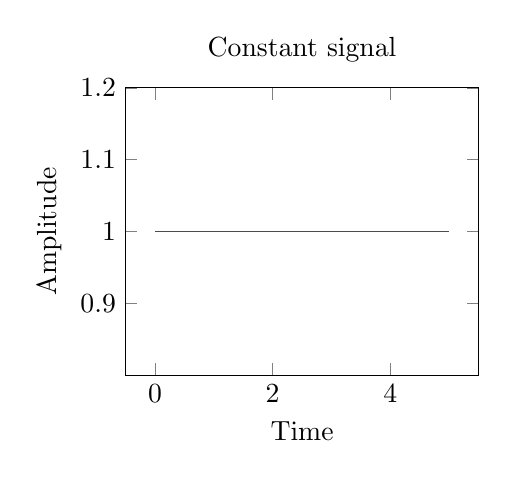
\begin{tikzpicture}
    % Signal constant
    \begin{axis}[
        width=0.5\textwidth,
        title=Constant signal,
        xlabel=Time,
        ylabel=Amplitude,
      ]
      \addplot[red, const plot] coordinates {(0, 1) (5, 1)};
    \end{axis}
  \end{tikzpicture}
\end{figure}

\subsubsection{Voltage, Current, and Resistance}

\subsubsection{Ohm's Law and Power}
text\par
\begin{figure}[!h]
  \centering
  \ifdefined\HCode
  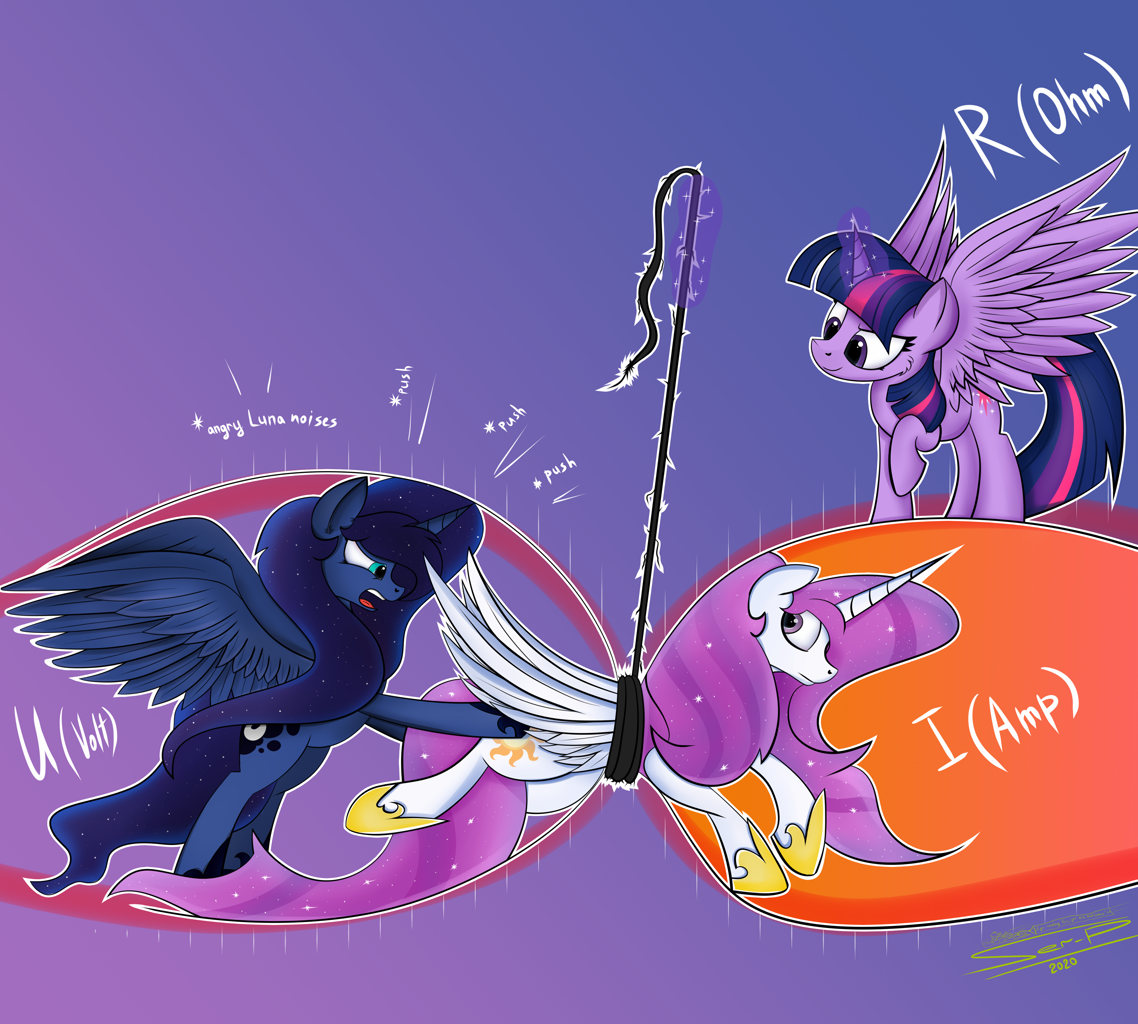
\includegraphics[height=45em,keepaspectratio]
  {src/assets/electricity_pony.png}
  \else
  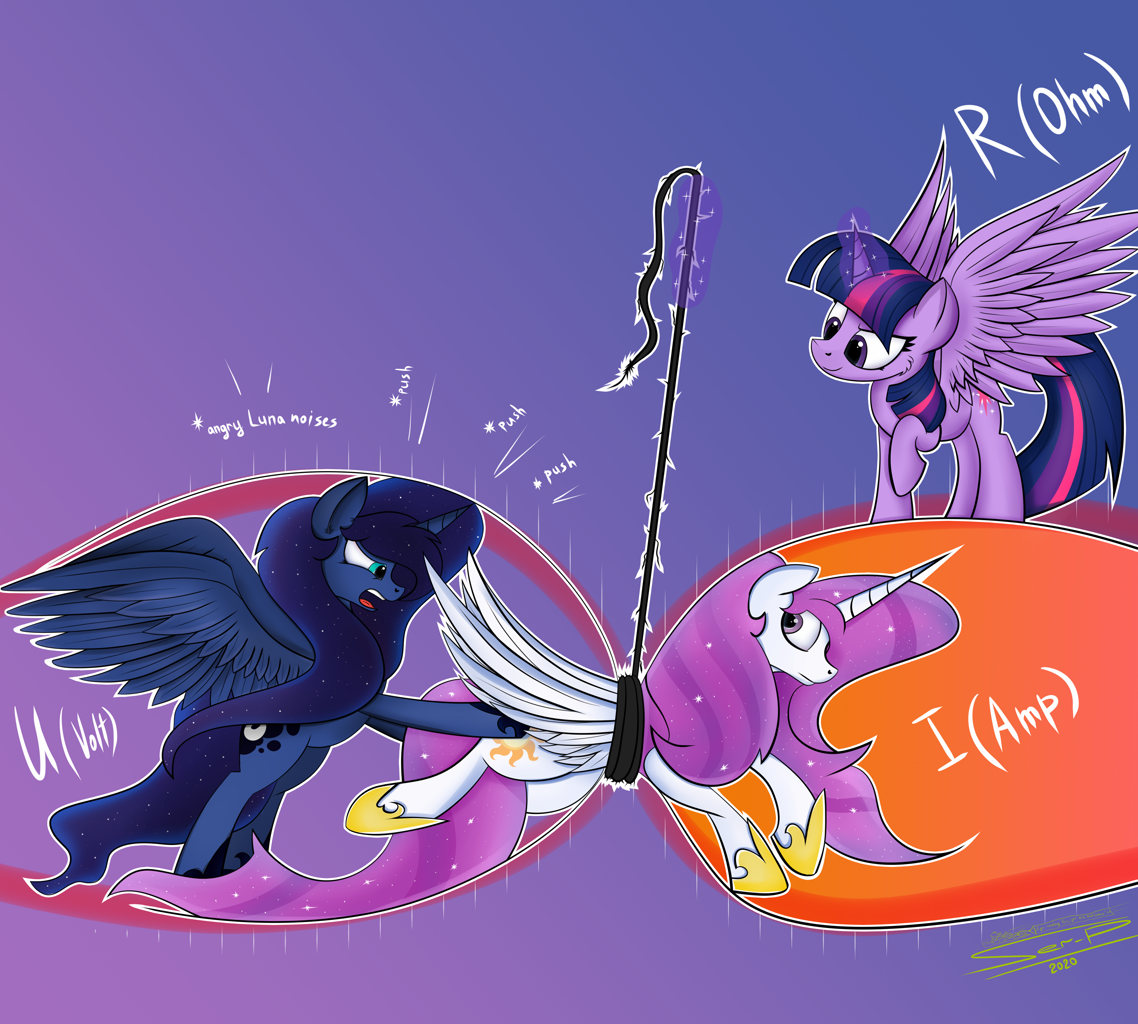
\includegraphics[height=0.7\textwidth,keepaspectratio]
  {src/assets/electricity_pony.png}
  \fi
  \caption{Electrical resistance explained with ponies.\\
  \textbf{Source:}\href{https://derpibooru.org/images/2461820?q=electrical+resistance}{derpibooru.org}}
\end{figure}
\subsection{Basic Components} \label{subsec:basic_components}
\subsubsection{Resistors}
\subsubsection{Capacitors}
\subsubsection{Inductors (Coil Inductance, Magnetic Flux)}
\subsubsection{Diodes}
\subsubsection{Transistors}
\subsection{Schematics and Symbols} \label{subsec:schematics_symbols}

\section{Analog and AC Circuits} \label{sec:analog_ac}
\subsection{AC Circuit Theory} \label{subsec:ac_circuit_theory}
\subsubsection{RLC Circuits}
\subsubsection{Impedance and Reactance}
\subsection{Filters and Frequency Response} \label{subsec:filters}
\subsection{Transformers and Electromagnetism} \label{subsec:transformers}
\subsection{Power Supplies and Power Electronics}
\label{subsec:power_electronics}

\section{Operational Amplifiers and Oscillators} \label{sec:opamps_oscillators}
\subsection{Operational Amplifiers} \label{subsec:opamps}
\subsubsection{Inverting and Non-Inverting Amplifiers}
\subsubsection{Feedback and Gain Control}
\subsection{Oscillators} \label{subsec:oscillators}
\subsubsection{RC Oscillators}
\subsubsection{LC Oscillators}

\section{Digital Electronics and Logic} \label{sec:digital_electronics}
\subsection{Number Systems} \label{subsec:number_systems}
\subsubsection{Binary}
\subsubsection{Hexadecimal}
\subsection{Boolean Algebra and Logic Gates} \label{subsec:boolean_logic}
\subsubsection{AND, OR, NOT, NAND, NOR Gates}
\subsection{Combinational Logic} \label{subsec:combinational_logic}
\subsubsection{Multiplexers}
\subsubsection{Encoders and Decoders}
\subsection{Sequential Logic} \label{subsec:sequential_logic}
\subsubsection{Flip-Flops}
\subsubsection{Counters}
\subsubsection{Registers}

\section{Electronic Systems and Control} \label{sec:systems_control}
\subsection{System Theory} \label{subsec:system_theory}
\subsubsection{Inputs and Outputs}
\subsubsection{Block Diagrams}
\subsection{Feedback Systems} \label{subsec:feedback}
\subsubsection{Open-Loop Control}
\subsubsection{Closed-Loop Control}

\section{Radio Frequency (RF) Foundations} \label{sec:rf_foundations}
\subsection{RF and Microwave Spectrum} \label{subsec:rf_spectrum}
\subsection{Electromagnetic Wave Propagation} \label{subsec:wave_propagation}
\subsubsection{Line-of-Sight Constraints}
\subsection{Transmission Line Basics} \label{subsec:transmission_lines}
\subsubsection{S-Parameters and dB Units}

\section{Transmission Lines and Waveguides} \label{sec:waveguides}
\subsection{Coaxial and Microstrip Lines} \label{subsec:coaxial_microstrip}
\subsection{Waveguide Theory} \label{subsec:waveguide_theory}
\subsubsection{Modes of Propagation}
\subsubsection{Cutoff Frequency}

\section{Microwave Components and Devices} \label{sec:microwave_components}
\subsection{Antennas and Resonators} \label{subsec:antennas_resonators}
\subsection{Microwave Sources} \label{subsec:microwave_sources}
\subsubsection{Klystron}
\subsubsection{Magnetron}
\subsubsection{Gunn Diode}
\subsubsection{Traveling-Wave Tube (TWT)}
\subsection{Passive Microwave Devices} \label{subsec:passive_microwave}
\subsubsection{Directional Couplers}
\subsubsection{E-Plane and H-Plane Tees}
\subsubsection{Rat-Race Junctions}

\section{Microwave Communication Systems} \label{sec:microwave_communications}
\subsection{Point-to-Point Microwave Links} \label{subsec:microwave_links}
\subsection{Satellite and Terrestrial Systems} \label{subsec:satellite_systems}
\subsection{Radar Principles} \label{subsec:radar}
\subsection{RF PCB Design Considerations} \label{subsec:rf_pcb}

\section{Microwave Measurements, Safety, and Standards}
\label{sec:microwave_measurements}
\subsection{Measurement Techniques} \label{subsec:measurement_techniques}
\subsubsection{Power, Attenuation, Phase}
\subsection{Microwave Radiation Safety} \label{subsec:microwave_safety}

\section{Advanced RF Topics} \label{sec:advanced_rf}
\subsection{Impedance Matching and Smith Chart}
\label{subsec:impedance_matching}
\subsection{Millimeter-Wave Systems} \label{subsec:mm_wave}
\subsubsection{Frequency Ranges and Applications}
\subsubsection{Atmospheric Attenuation}
\subsection{Wireless Power Transmission via Microwaves}
\label{subsec:wireless_power}

\newpage
\ifdefined\HCode
\else
\addcontentsline{toc}{section}{References}
\fi
\printbibliography

\end{document}
